\subsection*{2.1}
  % Implement the CE-CC amplifier shown below:
    \begin{figure}[h!]
        \centering
        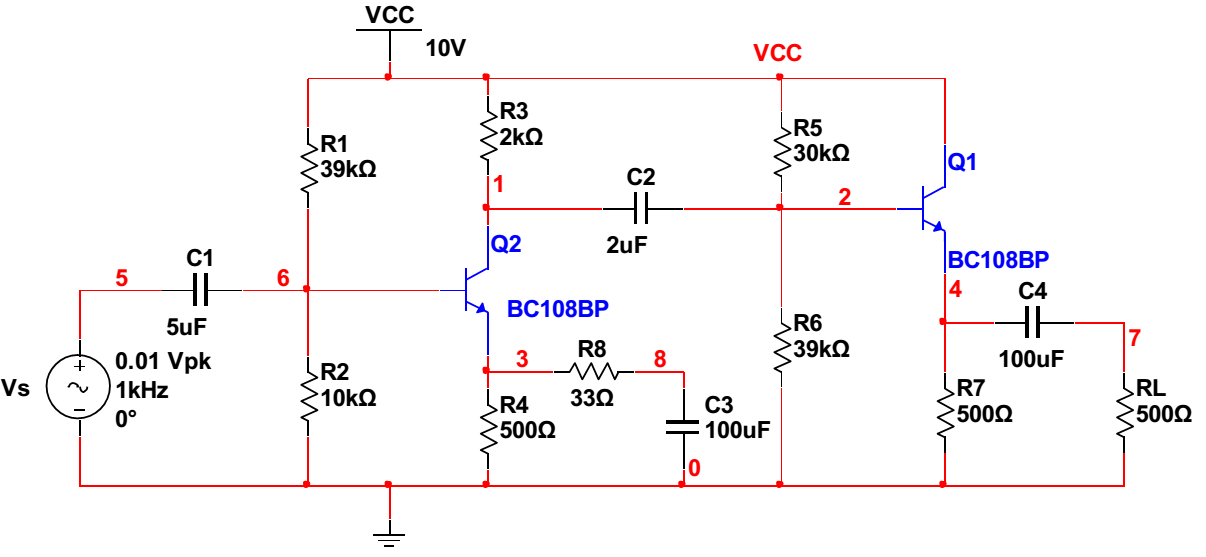
\includegraphics[width=6cm]{fig2-1.png}
        \captionof{figure}{The CE-CC amplifier to be implemented in Task 2.1}
    \end{figure}    

\subsection*{2.2}
  % Using  proper  simulation  techniques,  determine  the  following  parameters  of  the  circuit:
  % (i) Midband voltage gain,
  % (ii) Input resistance,
  % (iii) Output resistance,
  % (iv) Lower 3dB frequency,
  % (v) Upper 3dB frequency,
  % (vi)  Maximum  output  voltage  amplitude  for  which  the  total  harmonic  distortion  of  the
  % output signal is less than 5% at the input signal frequency of 1kHz. 

\subsection*{2.3}
  % Summarize  the  circuit  parameters  in  a  table  and  attach  relevant  plots.  Explain  the
  % simulation techniques that you exploited.
  